\documentclass{beamer}
\usepackage{fontspec}
\usepackage{xunicode}
\usepackage{xltxtra}
\usepackage{tikz}
\usetheme{/ULB}

\title{Merging and Sorting Partial Orders in the Decision Tree Model}
\author{Ooms Aurélien}
\institute{
\smallcaps{\Large Université Libre de Bruxelles}\\[0.442cm]
{\large Faculty of Science}\\[0.114cm]
{\large Department of Computer Science}\\[0.114cm]
}
\date{Academic Year 2013~-~2014}
\begin{document}

{
\setbeamertemplate{sidebar left}{}
%\setbeamertemplate{background canvas}{\tikz[remember picture,overlay]\node[opacity=1] at (current page.center) {\includegraphics[height=0.5\paperheight,keepaspectration,bb=70mm -160mm 105mm 46mm]{img/ulb}};}
\begin{frame}
\titlepage
\end{frame}
}

\section{The Model}
\subsection{Numbers}
\begin{frame}[c]{The Model}{Numbers}
\begin{figure}[hbtp]
\centering

\includegraphics[width=0.7\textwidth]{fig/number/cloud}
% \caption{Interesting Underwater Environment}
\end{figure}
\end{frame}

\subsection{Numbers Comparison}
\begin{frame}[c]{The Model}{Numbers Comparison}
\begin{figure}[hbtp]
\centering
\includegraphics[width=0.7\textwidth]{fig/number/comp}
% \caption{Human Underwater Observation}
\end{figure}
\end{frame}

\begin{frame}[c]{The Model}
\begin{figure}[hbtp]
\centering
\includegraphics[width=0.7\textwidth]{fig/number/put}
% \caption{Inevitable Damaging and Unexpected Behavior}
\end{figure}
\end{frame}

\begin{frame}[c]{The Model}
\begin{figure}[hbtp]
\centering
\includegraphics[width=0.7\textwidth]{fig/number/close}
% \caption{Automated Fish Filming}
\end{figure}
\end{frame}

\begin{frame}[c]{The Model}
\begin{figure}[hbtp]
\centering

\includegraphics[width=0.7\textwidth]{fig/box/cloud}
% \caption{Automated Fish Filming}
\end{figure}
\end{frame}

\begin{frame}[c]{The Model}
\begin{figure}[hbtp]
\centering
\includegraphics[width=0.7\textwidth]{fig/box/comp}
% \caption{Automated Fish Filming}
\end{figure}
\end{frame}


\begin{frame}[c]{The Model}
\begin{figure}[hbtp]
\centering
\includegraphics[width=0.7\textwidth]{fig/box/ask}
% \caption{Automated Fish Filming}
\end{figure}
\end{frame}

\begin{frame}[c]{The Model}
\begin{figure}[hbtp]
\centering
\includegraphics[width=0.7\textwidth]{fig/box/yes}
% \caption{Automated Fish Filming}
\end{figure}
\end{frame}

\begin{frame}[c]{The Model}
\begin{figure}[hbtp]
\centering
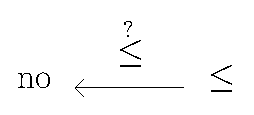
\includegraphics[width=0.7\textwidth]{fig/box/no}
% \caption{Automated Fish Filming}
\end{figure}
\end{frame}

\section{Problematic}

%problematic
\begin{frame}[c]{Problematic}

	\center Automated Solution: advantages \& intricacy
	\bigskip
	\pause
	\begin{columns}
 		\begin{column}{0.5\textwidth}
			\center Advantages
			\begin{itemize}
				\item Continuous acquisition
				\item Timely maintenance
				\item Reduced cost
			\end{itemize}
		\end{column}
		\pause
		\begin{column}{0.5\textwidth}
			\center Intricacy
			\begin{itemize}
				\item Explosion of collected data
				\item Strength of material
				\item IT solution needed
			\end{itemize}
		\end{column}
	\end{columns}
\end{frame}

\section{Example}

\begin{frame}[c]{Example}
1 min. of video
\begin{columns}
	\begin{column}{0.5\textwidth}
			\begin{itemize}
				\item Watch
				\item Classify
				\item Annotate
			\end{itemize}
	\end{column}
	\pause
	\begin{column}{0.5\textwidth}
			\begin{itemize}
				\item $\approx$ 15 min.
			\end{itemize}
	\end{column}
\end{columns}
	\pause
\bigskip	
\center Fully analyse a year of existing videos would take approximately \textbf{15 years}.
\end{frame}

\section{Methodology}

%methodology
\begin{frame}[c]{Methodology}
\center
\begin{itemize}
\item the frame analysis
\item the fish detection
\item the tracking
\end{itemize}
\end{frame}

\begin{frame}[c]{Methodology : Frame Analysis}
\center
Video Stream $=$ an images flow $I_{0:t}$ at a rate $\tau$ \\

\includegraphics[height=0.25\textheight]{fig/number/cloud} \\
\pause
\bigskip
Each image $i_k$ is called a \textit{frame}, each \textit{frame} is a matrix $n*m$ 
\[ \left( \begin{array}{ccc}
p_{0,0} & \ldots & p_{n,0} \\
\vdots & \ddots & \vdots \\
p_{0,m} & \ldots & p_{n,m} \end{array} \right)\] 
\end{frame}

\begin{frame}[c]{Methodology : Frame Analysis}
\center
Whole \textbf{Image} $-$ \textit{static} \textbf{Background} $=$ moving \textbf{Foreground}\\
\center 
\includegraphics[width=0.7\textwidth]{fig/number/cloud} \\
\end{frame}


\begin{frame}[c]{Methodology : Frame Analysis}
\center \textbf{Accumulating} background\\

$$
\alpha := learning\ rate
$$
$$
background_t = (1-\alpha)\ background_{t-1} + \alpha\ i_t
$$
$$
foreground_t = i_t - background_t
$$

\end{frame}


\begin{frame}[c]{Methodology : Fish Detection}
\center \textbf{Color} comparison\\
\begin{figure}[hbtp]
\centering

\includegraphics[width=0.7\textwidth]{fig/number/cloud}
\pause
\center We \textbf{can't} use this!
\end{figure}
\end{frame}

\begin{frame}[c]{Methodology : Fish Detection}
\center Target \textbf{features} extraction\\
\begin{figure}[hbtp]
\centering

\includegraphics[width=0.7\textwidth]{fig/number/cloud}
% \caption{Invariants Features}
\end{figure}
\end{frame}

\begin{frame}[c]{Methodology : Fish Detection}
\center \textbf{Contours} \\
\begin{figure}[hbtp]
\centering

\includegraphics[width=0.7\textwidth]{fig/number/cloud}
\end{figure}
\end{frame}

\begin{frame}[c]{Methodology : Fish Detection}
\center An \textbf{invariant} point \\
\begin{figure}[hbtp]
\centering

\includegraphics[width=0.7\textwidth]{fig/number/cloud}
\end{figure}
\end{frame}


\begin{frame}[c]{Methodology : Fish Detection}
\center Matching \textbf{invariant} points \\

$$
\delta := euclidian\ distance
$$
$$
\epsilon := distance\ threshold
$$
$$
p_t = p_{t-1}\ \text{if}\ \delta(p_t, p_{t-1}) < \epsilon
$$

\end{frame}


\begin{frame}[c]{Methodology : Tracking}
\center Tracking $=$ identifying a set of pixels \\as \textit{identical} between 2 frames\\
\begin{figure}[hbtp]
\centering

\includegraphics[width=0.7\textwidth]{fig/number/cloud}
% \caption{Target's Features Tracking}
\end{figure}
\end{frame}

\end{document}